\subsection{Universidad de San Petersburgo}

Resultados obtenidos en el monitoreo:\\

\smallskip
\begin{tabular}{| l | c | c | c | c |}
\hline
Hop & IP &  RTT promedio (s)  & deltaRTT promedio & Ubicacion\\ 
\hline
1 & 192.168.11.1 & 0.01142361429 & 0.01142361429 & Argentina, Buenos Aires\\
\hline
2 & 10.21.128.1 & 0.0283621417152 & 0.0169385274251 & Argentina, Buenos Aires\\
\hline
3 & 10.242.0.201 & 0.0378749105665 & 0.00951276885139 & Argentina, Buenos Aires\\
\hline
4 & 195.22.220.33 & 0.0143795543247 & 0 & Italy\\
\hline
5 & 195.22.220.32 & 0.292960882187 & 0.278581327862 & Italy\\
\hline
6 & 89.221.41.171 & 0.152727180057 & 0 & Italy\\
\hline
7 & 89.221.41.171 & 0.156960460875 & 0.00423328081767 & Italy\\
\hline
8 & 154.54.9.17 & 0.202791770299 & 0.0458313094245 & United States\\
\hline
9 & 154.54.80.41 & 0.21254154614 & 0.00974977584112 & United States\\
\hline
10 & 66.28.4.237 & 0.168935351902 & 0 & United States, Pasadena\\
\hline
11 & 154.54.29.222 & 0.251122385263 & 0.0821870333619 & United States\\
\hline
12 & 154.54.42.77 & 0.316137870153 & 0.0650154848893 & United States\\
\hline
13 & 154.54.45.162 & 0.327892038557 & 0.0117541684045 & United States\\
\hline
14 & 154.54.45.2 & 0.255609459347 & 0 & United States\\
\hline
15 & 38.88.196.186 & 0.270633061727 & 0.0150236023797 & United States, Los Angeles\\
\hline
16 & 101.4.117.169 & 0.435372935401 & 0.164739873674 & China, Beijing\\
\hline
17 & 101.4.117.97 & 0.467933893204 & 0.0325609578027 & China, Beijing\\
\hline
18 & 101.4.112.105 & 0.437322590086 & 0 & China, Beijing\\
\hline
19 & 101.4.118.94 & 0.43985332383 & 0.0025307337443 & China, Beijing\\
\hline
20 & 101.4.112.90 & 0.435603486167 & 0 & China, Beijing\\
\hline
21 & 101.4.117.81 & 0.413042836719 & 0 & China, Beijing\\
\hline
22 & 202.112.41.178 & 0.405184189479 & 0 & China, Shanghai\\
\hline
23 & 202.112.41.182 & 0.394645796882 & 0 & China, Shanghai\\
\hline
24 & 162.105.252.133 & 0.488684309853 & 0.0940385129717 & China, Beijing\\
\hline
\end{tabular}
\bigskip

\textbf{Paquetes enviados: 145 / Paquetes no respondidos: 14}\\

\textbf{Dos outliers, hops: 10 y 11}\\

Algo extraño es que según la herramienta de geolocalización los saltos 7 a 9 están ubicados en España, pero sus RTT promedio no varían demasiado de las de Argentina. Para explicar este fenómeno se nos ocurrieron las siguientes hipótesis:
\begin{itemize}
\item La herramienta de geolocalización falló y en realidad los host se encuentran en Argentina.
\item Según investigamos hay un enlace intercontinental con fibra óptica que va desde Las Toninas hasta Portugal, quizás esta opción es mejor para luego pasar a EEUU.
\item Las IPs están registradas en España (corresponden a Telefónica España) pero tienen servidores en Argentina o algún país limítrofe.
\end{itemize}

A falta de más datos preferimos estatar todas las hipótesis ya que no pudimos terminar de decidirnos por ninguna.\\

En el hop 10 aumenta el RTT promedio (y es un outlier) ya que es entonces en donde suponemos viaja hasta Estados Unidos. El hop 11 no varía demasiado respecto al 10 y a pesar de ser un outlier no es un salto importante, no se viaja intercontinentalmente, como en el próximo (el hop 12) en el cual se llega hasta Irlanda.\\

Después de ese salto los RTT se mantienen entre si, ninguno se destaca, hasta llegar a destino. Con esto vemos que el método Cimbala en este caso falla al detectar el salto intercontinental.\\

A continuación mostramos un gráfico con los RTT entre saltos y otro con los ZRTT\footnote{ZRTT = $(X_i - \bar{X}) / S$}  entre saltos. También así el planisferio con los saltos graficados.

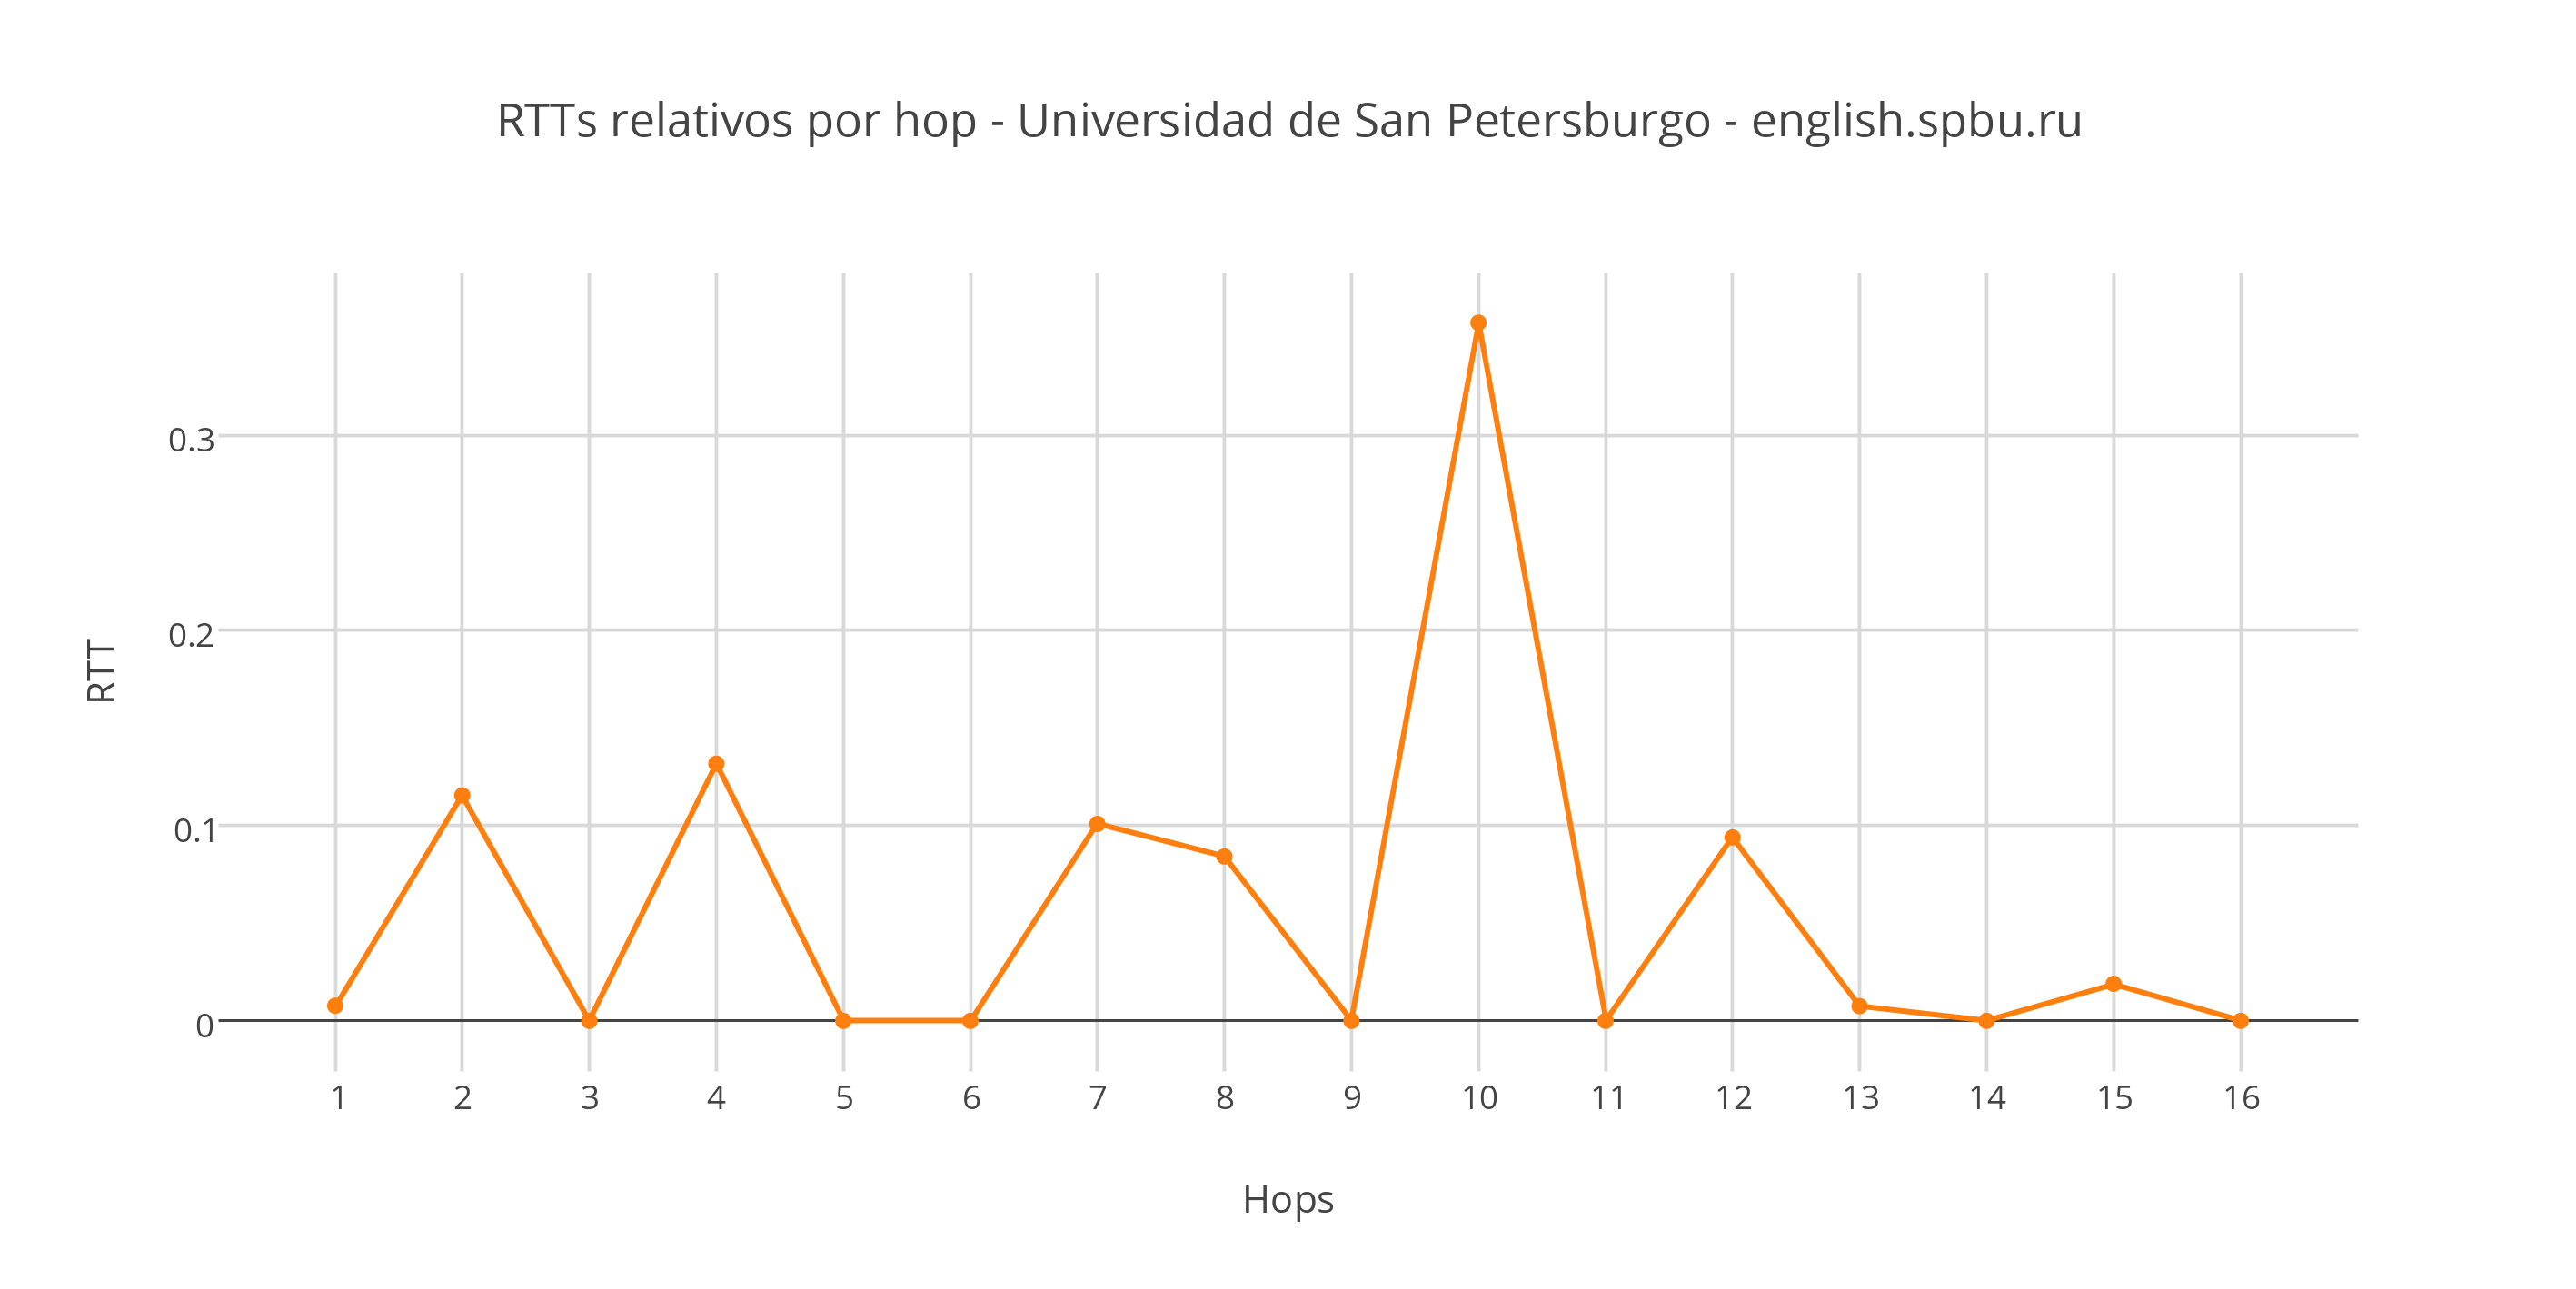
\includegraphics[scale=0.65]{imagenes/rusia/RTTs.png} 

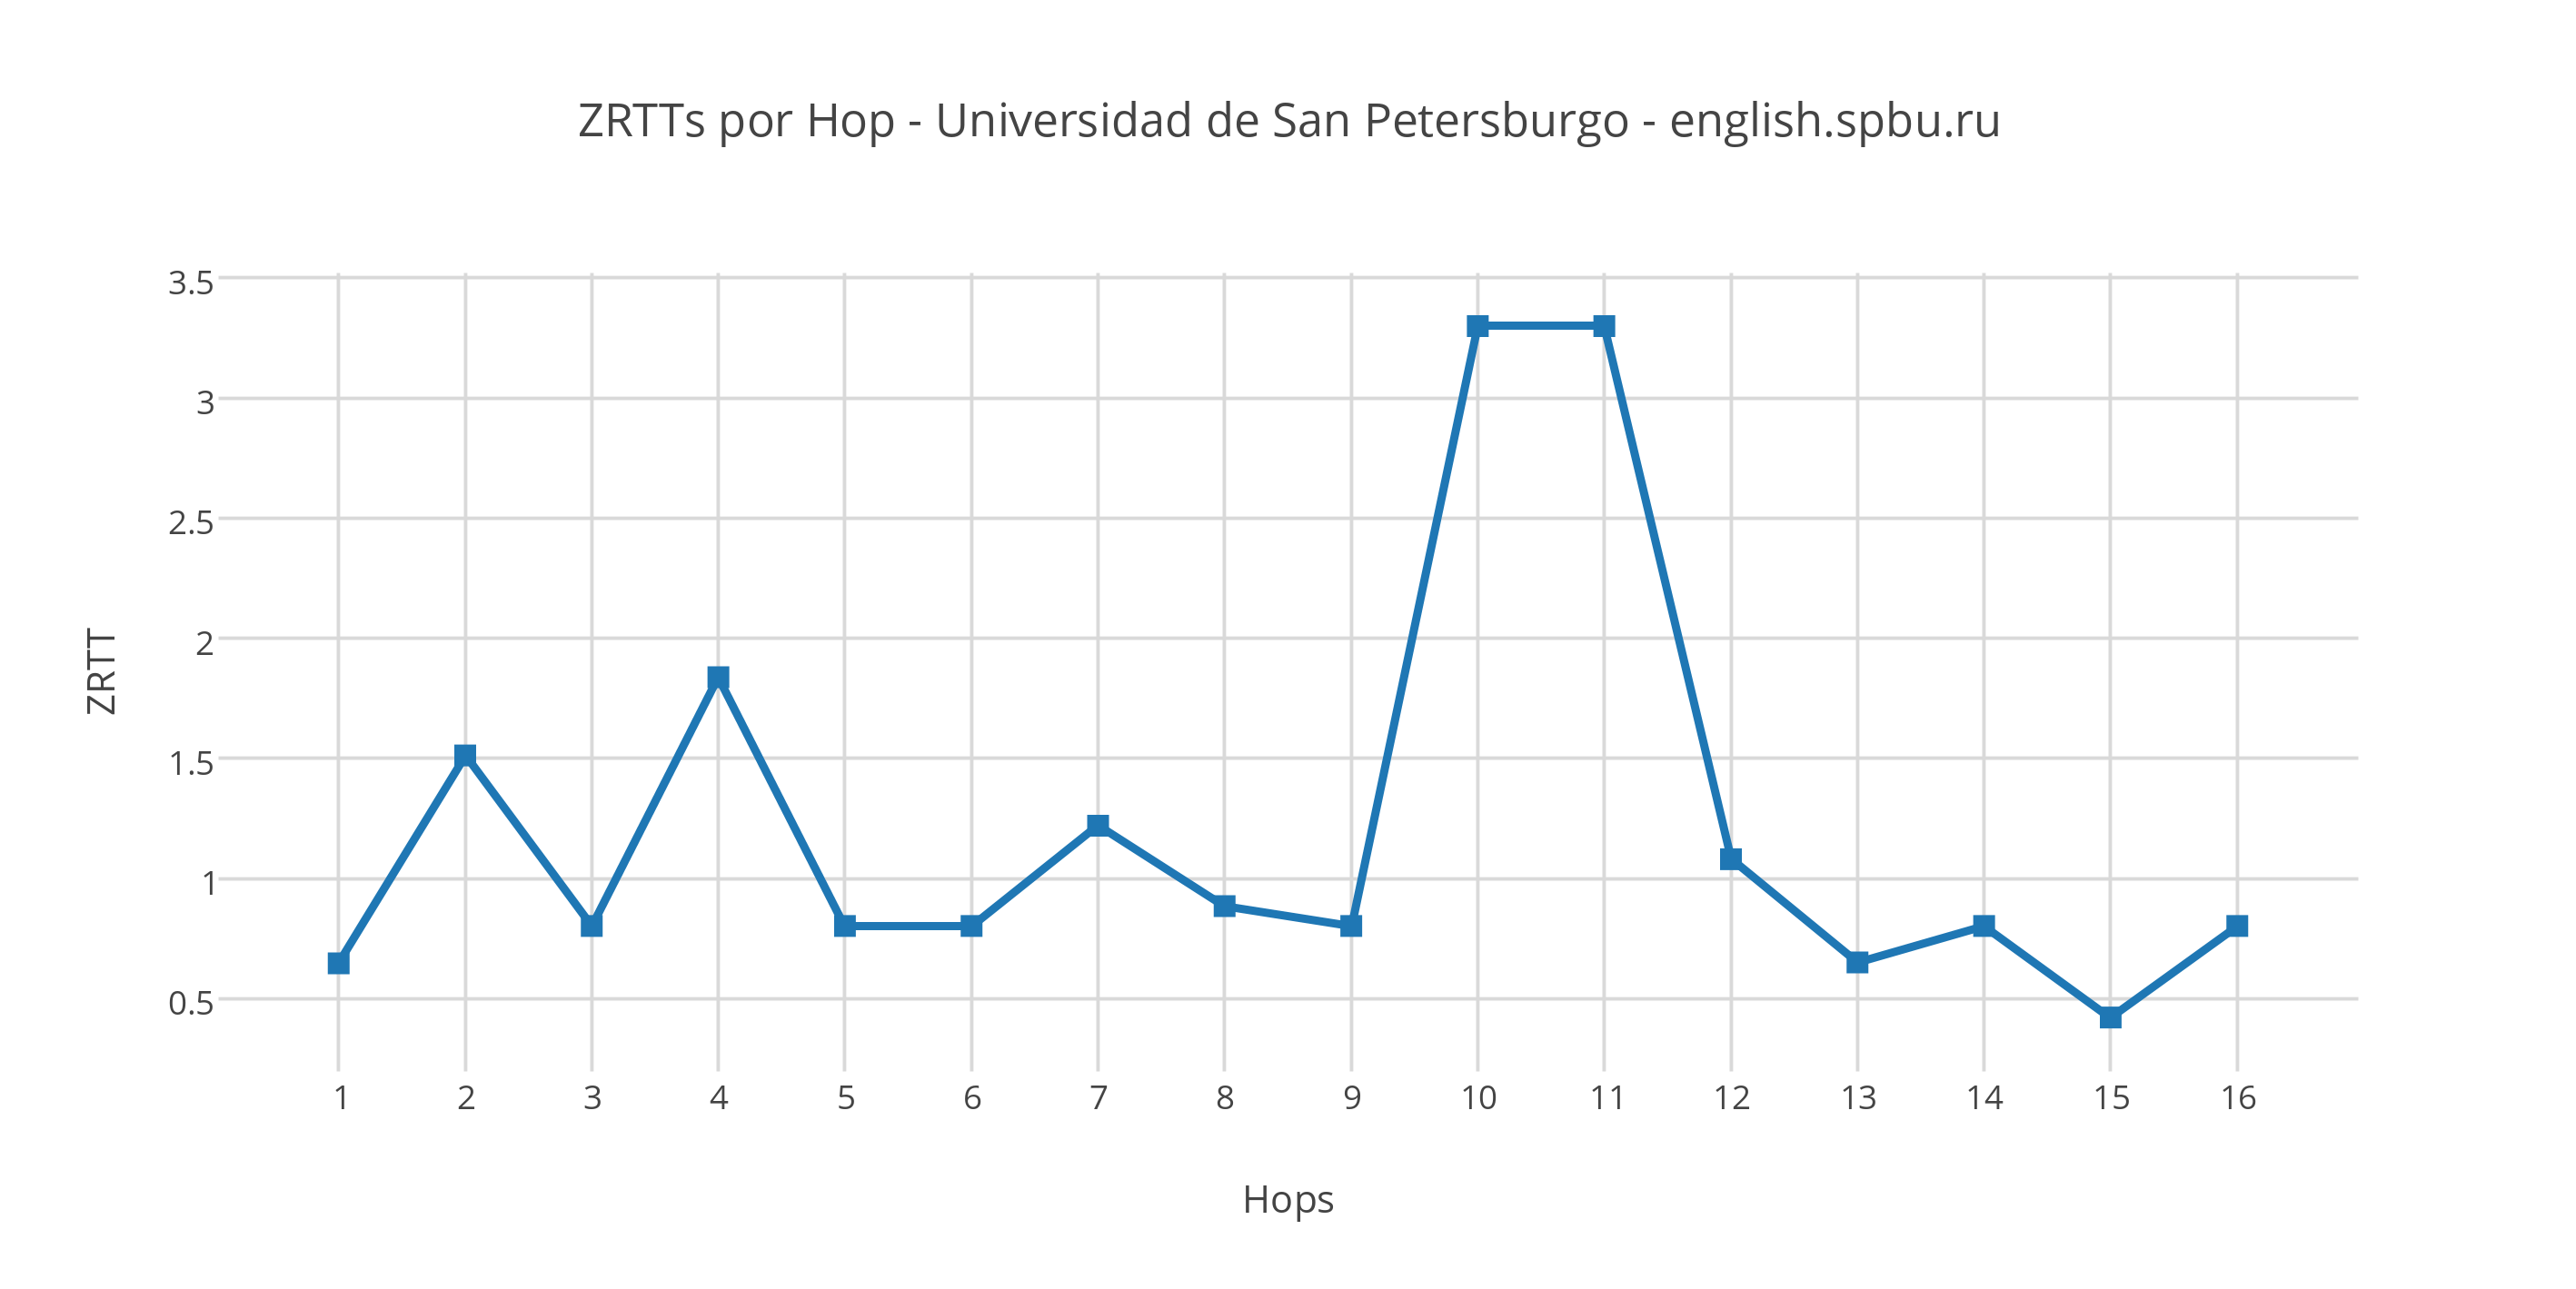
\includegraphics[scale=0.65]{imagenes/rusia/ZRTTs.png} 

\begin{center}
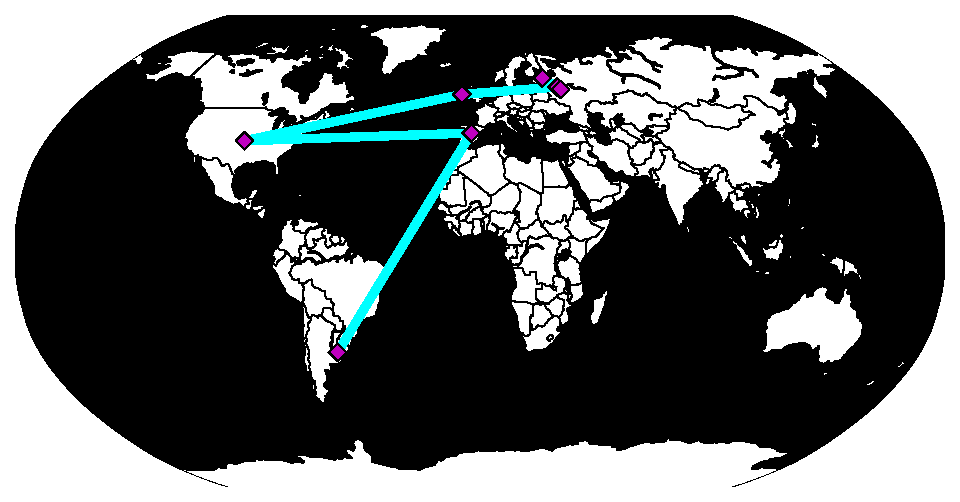
\includegraphics[scale=0.8]{imagenes/rusia/rusia.pdf} 
\end{center}
